% CO3133 Assignment 3 — M1 Dataset Proposal (LaTeX report edition)
% Scientific XeLaTeX style aligned with the M2 report.
% Evidence and experiment plans are the historical M1 record prepared 4 November 2026.
% No M2/M3 model results or training claims appear in this proposal.
% Compile twice with XeLaTeX; figures are native PGFPlots/TikZ vectors.
\documentclass[11pt,a4paper]{article}
\usepackage[a4paper,left=23mm,right=23mm,top=23mm,bottom=22mm,headheight=14pt,headsep=7mm,footskip=11mm]{geometry}
\usepackage{fontspec}
\IfFileExists{/usr/share/fonts/truetype/liberation/LiberationSerif-Regular.ttf}{%
  \setmainfont[Path=/usr/share/fonts/truetype/liberation/,BoldFont=LiberationSerif-Bold.ttf,ItalicFont=LiberationSerif-Italic.ttf,BoldItalicFont=LiberationSerif-BoldItalic.ttf]{LiberationSerif-Regular.ttf}%
}{\setmainfont{TeX Gyre Termes}}
\usepackage{unicode-math}
\IfFileExists{/usr/share/texmf/fonts/opentype/public/lm-math/latinmodern-math.otf}{%
\setmathfont[Path=/usr/share/texmf/fonts/opentype/public/lm-math/]{latinmodern-math.otf}%
}{\setmathfont{Latin Modern Math}}
\usepackage{microtype,setspace}
\setstretch{1.055}
\usepackage{amsmath}
\usepackage{booktabs,tabularx,array,multirow,longtable}
\usepackage{caption}
\captionsetup{font=small,labelfont=bf,justification=justified,singlelinecheck=false,skip=5pt}
\usepackage{titlesec}
\titleformat{\section}{\fontsize{12}{14}\selectfont\bfseries}{\thesection.}{0.6em}{}
\titleformat{\subsection}{\fontsize{11}{13}\selectfont\bfseries}{\thesubsection}{0.7em}{}
\titlespacing*{\section}{0pt}{11pt}{5pt}
\titlespacing*{\subsection}{0pt}{8pt}{3pt}
\usepackage{fancyhdr}
\pagestyle{fancy}
\fancyhf{}
\fancyhead[L]{\footnotesize CO3133 \;|\; Group Goat \;|\; Assignment 3 -- Milestone 1}
\fancyhead[R]{\footnotesize Dataset proposal}
\fancyfoot[L]{\footnotesize 4 November 2026}
\fancyfoot[R]{\footnotesize Page \thepage}
\renewcommand{\headrulewidth}{0.3pt}
\renewcommand{\footrulewidth}{0pt}
\setlength{\parindent}{0pt}
\setlength{\parskip}{3pt plus 0.6pt minus 0.3pt}
\setlength{\tabcolsep}{5pt}
\renewcommand{\arraystretch}{1.12}
\usepackage{enumitem}
\setlist{nosep,leftmargin=1.5em}
\usepackage{float}
\usepackage[section]{placeins}
\usepackage{xcolor}
\definecolor{imageblue}{HTML}{4477AA}
\definecolor{textorange}{HTML}{CC6677}
\definecolor{fusionteal}{HTML}{009988}
\definecolor{gridgray}{HTML}{D6DCE2}
\definecolor{softgray}{HTML}{F1F4F7}
\usepackage{tikz}
\usepackage{pgfplots}
\pgfplotsset{compat=1.18}
\usepgfplotslibrary{groupplots}
\usetikzlibrary{arrows.meta,positioning,calc}
\usepackage[hidelinks]{hyperref}
\usepackage{xurl}
\urlstyle{same}
\usepackage{lastpage}
\newcommand{\primary}{\texttt{filtered\_original}}
\newcommand{\smallnote}[1]{\par\vspace{-3pt}{\footnotesize\itshape #1}\par}
\begin{document}
\begin{center}
{\footnotesize\bfseries HO CHI MINH CITY UNIVERSITY OF TECHNOLOGY -- VNU-HCM}\\[2pt]
{\footnotesize Faculty of Computer Science and Engineering \;|\; Deep Learning and Its Applications (CO3133)}\\[2pt]
{\footnotesize Semester 261 \;|\; Instructor: Lê Thành Sách}\\[13pt]
{\Large\bfseries Humanitarian Image and Text Classification\\[2pt]
with Gated Fusion}\\[7pt]
{\normalsize\bfseries Assignment 3, Milestone 1 -- Dataset Proposal}\\[5pt]
{\normalsize Group Goat}\\[3pt]
{\small Nguyễn Huỳnh Nam Quốc (2453089) -- Assignment 3 lead, 100\% contribution}\\[2pt]
{\small Hoàng Trọng Huy Minh (2452743), 0\% \;|\; Võ Lê Thành Triệu (2453297), 0\%}\\[3pt]
{\small Prepared 4 November 2026 \;|\; M1 due 18 November 2026, 23:59 GMT+7}
\end{center}
\vspace{5pt}
\noindent{\bfseries Abstract.}\;
We propose five-class humanitarian classification of aligned crisis-related tweets and their attached images using an explicitly mirror-derived subset of CrisisMMD v2.0. A completed pre-experiment data audit examined 8,079 paired records; the locked \primary{} evaluation protocol retains 7,938 pairs (6,001 train, 986 development, and 951 test) after excluding 141 records for annotation discrepancies, image placeholders, and duplicate/leakage-related components. The plan compares frozen ResNet-18 image features, frozen DistilBERT text features, concatenation fusion, and learned scalar-gated fusion under shared controls. Macro-F1 is the principal metric; controlled gate ablation, paired error inspection, and measured compute accounting are planned. The source archive's exact equivalence to the third-party mirror is unverified. This proposal documents the dataset, evaluation design, and resource assumptions only: \emph{no classifier has been trained, and no model result is reported here}.

{\footnotesize\textbf{Keywords:} multimodal learning; CrisisMMD; image--text alignment; leakage-aware splits; gated fusion; dataset proposal.}

\section{Research Problem and Objectives}
Crisis-related social-media content often contains both text and images. We plan to classify each tweet--image pair into one of five humanitarian categories; a tweet with multiple attached images contributes multiple records. CrisisMMD provides a research corpus for studying disaster-related information, but its historical event mix and user-generated content limit deployment claims \cite{alam2018,ofli2020}. The prediction unit is a paired observation, not an independent image or tweet.

\textbf{Research question.} Under fixed frozen encoders and leakage-controlled partitions, does learned gated fusion improve macro-F1 relative to simple concatenation and the two unimodal models, and which modality interactions explain any gains or failures?

The objectives are to establish fair image-only and text-only baselines, compare them with concatenation and learned gating, isolate the contribution of gating via ablation, and explain paired classification errors and compute cost. Superior multimodal performance is a \emph{hypothesis}, not a promised outcome. This M1 proposal is weighted at 15\% of Assignment 3 in the course handbook \cite{handbook2026}.

\textbf{Submission basis.} The group reports that the instructor waived prior dataset approval for this group; this is not presented as a formal approval decision. The present document records the M1 state as of 4 November 2026, before model implementation.

\section{Dataset Identity and Provenance}
The base resource is QCRI CrisisMMD v2.0. We use a custom five-class derivative of the agreed-label humanitarian configuration from the third-party \texttt{pranitchawla/crisismmd-mteb} mirror, not the complete eight-class QCRI dataset \cite{qcri,mirror}. The audited mirror contains 8,079 image--text pairs; the selected primary set contains 7,938. Each pair has a five-class target plus source image/tweet identifiers; modality annotations and confidence metadata are available in primary source records.

The pinned primary QCRI revision is \texttt{10a5626ba112ab9c50369c473a2062bcf205d708}; the pinned mirror revision is \texttt{a935fda3cee8a5250746a8d1d6278214d615cc89}. Exact payloads and checksums are recorded in the accompanying provenance JSON files and \path{A3-M1/DATASET_LOCK.json}. The upstream CC BY-NC-SA 4.0 terms require attribution, identification of derivative changes, noncommercial use and appropriate share-alike compliance. We infer no additional rights over underlying media.

The original agreed-label ZIP returned HTTP 403 during the prior audit, so byte-for-byte equivalence between the accessible mirror and original archive is \emph{not} established. A 245/245 image-byte match concerns only the specifically checked subset; it does not prove overall archive identity.

\section{Verified Paired Samples and Preliminary EDA}
\subsection{Locked sample composition}
The completed validation/remediation evidence establishes 7,938 retained pairs spanning 7,103 distinct tweet IDs and 7,071 connected groups. All five humanitarian classes remain represented. The partition is fixed at 6,001 training, 986 development and 951 test records. Table~\ref{tab:classcounts} describes the exact locked primary population.
\begin{table}[htbp]
\centering\small
\caption{Measured class counts in the locked \primary{} protocol (source: published remediation class-count records).}
\label{tab:classcounts}
\begin{tabularx}{\linewidth}{@{}>{\raggedright\arraybackslash}Xrrrr@{}}
\toprule
Humanitarian class (ID) & Train & Dev & Test & Total \\
\midrule
Affected individuals (0) & 71 & 9 & 9 & 89 \\
Infrastructure and utility damage (1) & 601 & 80 & 81 & 762 \\
Rescue volunteering or donation effort (2) & 901 & 148 & 126 & 1,175 \\
Other relevant information (3) & 1,247 & 235 & 235 & 1,717 \\
Not humanitarian (4) & 3,181 & 514 & 500 & 4,195 \\
\midrule
\textbf{Total} & \textbf{6,001} & \textbf{986} & \textbf{951} & \textbf{7,938} \\
\bottomrule
\end{tabularx}
\end{table}
\textbf{Label mapping.} Injured/dead and missing/found people are combined into \emph{affected individuals}; vehicle damage is combined with infrastructure and utility damage. Other class meanings are unchanged. Primary modality agreement is checked \emph{before} these merges, and remediation does not silently relabel targets.

\begin{figure}[htbp]
\centering
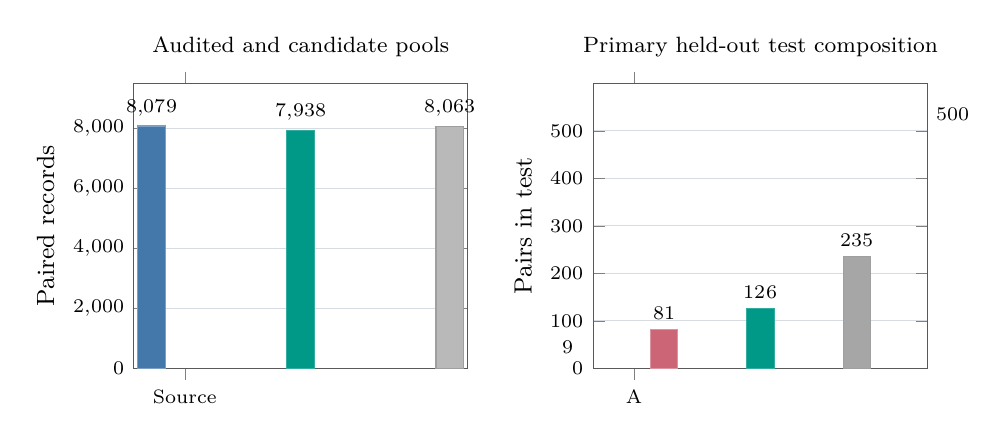
\begin{tikzpicture}
\begin{groupplot}[
  group style={group size=2 by 1,horizontal sep=1.6cm},
  height=5.2cm,width=0.48\linewidth,
  ybar,
  axis line style={black!65},
  tick label style={font=\scriptsize},label style={font=\small},
  ymajorgrids,grid style={draw=gridgray,thin},
  nodes near coords,nodes near coords style={font=\scriptsize},
  xtick=data]
\nextgroupplot[title={Audited and candidate pools},title style={font=\footnotesize},ylabel={Paired records},symbolic x coords={Source,Primary,Backup},xticklabels={Source,Primary,Backup},ymin=0,ymax=9500,scaled y ticks=false,ytick={0,2000,4000,6000,8000},xticklabel style={font=\scriptsize},enlarge x limits=0.22]
\addplot[fill=imageblue,draw=imageblue!70] coordinates {(Source,8079)};
\addplot[fill=fusionteal,draw=fusionteal!80] coordinates {(Primary,7938)};
\addplot[fill=gray!55,draw=gray!75] coordinates {(Backup,8063)};
\nextgroupplot[title={Primary held-out test composition},title style={font=\footnotesize},ylabel={Pairs in test},symbolic x coords={A,I,R,O,N},ymin=0,ymax=600,ytick={0,100,200,300,400,500},enlarge x limits=0.16]
\addplot[fill=imageblue,draw=imageblue!70] coordinates {(A,9)};
\addplot[fill=textorange,draw=textorange!70] coordinates {(I,81)};
\addplot[fill=fusionteal,draw=fusionteal!80] coordinates {(R,126)};
\addplot[fill=gray!70,draw=gray!75] coordinates {(O,235)};
\addplot[fill=imageblue!65!black,draw=imageblue!65!black] coordinates {(N,500)};
\end{groupplot}
\end{tikzpicture}
\caption{Dataset counts documented at M1. Left: source pool (8,079), selected \primary{} (7,938), and backup-only repartition (8,063; not selected using model scores). Right: the five class counts in the locked primary test split (A = affected, I = infrastructure, R = rescue/donation, O = other relevant, N = not humanitarian). The charts summarize previously audited counts, not model performance.}
\label{fig:remediation}
\end{figure}

\subsection{Preliminary source-pool input profiles}
Table~\ref{tab:inputprofile} is measured on the \emph{original 8,079-pair pool}, not recomputed for the filtered primary set. Word counts are whitespace-delimited and are \emph{not} DistilBERT subtoken counts.
\begin{table}[htbp]
\centering\small
\caption{Preliminary original-pool input statistics (not measurements on the filtered set).}
\label{tab:inputprofile}
\begin{tabularx}{\linewidth}{@{}>{\raggedright\arraybackslash}Xrr>{\raggedright\arraybackslash}X@{}}
\toprule
Original split & Median words & 95th percentile & Median image width / height \\
\midrule
Train (6,126) & 14 & 20 & 900 / 675 px \\
Dev (998) & 14 & 20 & 869.5 / 641 px \\
Test (955) & 14 & 20 & 864 / 635 px \\
\bottomrule
\end{tabularx}
\end{table}
The original audit decoded all 8,079 images and found no missing/corrupt files or empty texts; primary ID/path joins passed. Nevertheless, nine \emph{decodable image placeholders} were separately identified and removed. There were 652 heuristic text-encoding flags and 24 images with one side below 64 pixels in the original pool. These are warning flags, not confirmed semantic errors, and their filtered-population counts were not recomputed.

\section{Cross-Modal Alignment, Exclusions, and Split Protocol}
Each image ID/path is linked to a tweet ID, tweet text, and source event in pinned primary records. The image--text samples are attachments from the same posts, not random pairings between independent datasets \cite{qcri,mirror}. Linkage does not establish that every pictured location or textual claim is true.

A previous visual check found two compatible training examples: \texttt{904472503850082305\_0} (a flooded roadway with a Harvey flood-impact tweet) and \texttt{909878988407033857\_1} (animal transport crates alongside a post about moving shelter dogs). These illustrate \emph{pair compatibility} but do not establish dataset-wide semantic correctness.

\begin{table}[htbp]
\centering\small
\caption{Disjoint exclusions from the original 8,079-pair mirror. Total exclusions: 141; retained: 7,938.}
\label{tab:exclusions}
\begin{tabularx}{\linewidth}{@{}>{\raggedright\arraybackslash}Xrrrr@{}}
\toprule
Reason & Train & Dev & Test & Total \\
\midrule
Primary annotation discrepancy & 7 & 0 & 0 & 7 \\
Verified missing-image placeholder & 4 & 1 & 4 & 9 \\
Duplicate/leakage-related component member & 114 & 11 & 0 & 125 \\
\midrule
\textbf{Total} & \textbf{125} & \textbf{12} & \textbf{4} & \textbf{141} \\
\bottomrule
\end{tabularx}
\end{table}
\textbf{Annotation uncertainty.} The seven quarantined training targets are labelled \texttt{not\_humanitarian} by the mirror and QCRI humanitarian JSON/image fields, whereas the primary event TSV text fields label them \texttt{other\_relevant\_information}. IDs, text, and paths matched in the prior investigation. Their discrepancy remains unresolved; confidence fields do not justify silent relabelling.

\textbf{Leakage-control procedure (completed before model experiments).}
\begin{enumerate}[label=\arabic*.,itemsep=2pt]
\item Build connected components from shared tweet IDs, identical image bytes/pixels, raw and normalized text hashes, and 81 visually confirmed duplicate/shared-asset candidate edges.
\item Apply the audited text normalization: HTML unescape, Unicode NFKC and casefold, remove URLs, leading retweet/mention prefixes and mentions, and join Unicode word tokens. Identical normalized inputs are conservatively grouped, though this does not imply every such post has the same semantics.
\item Quarantine the seven discrepant rows and nine confirmed placeholders. For a component spanning eligible splits, retain only rows from the highest-priority existing split (test $>$ dev $>$ train); exclude lower-priority members without moving retained records.
\item Lock all retained row IDs, original splits, labels and image/text content hashes in the primary manifests. The primary filter is deterministic and needs no split seed; whole tweet/identity components remain in one partition.
\end{enumerate}

The previous remediation traced all 17 exact-image cross-split groups (54 records), and reviewed 134 perceptual-hash candidates: 70 duplicates, 11 shared-asset variants, 38 distinct observations and 15 placeholder edges (nine actual placeholder rows). Similar advisory graphics from different source observations were not automatically merged. Fifty-one candidate-protocol checks passed, and 26 resulting files had identical rerun hashes. This is dataset verification, \emph{not} trained-model validation.

\textbf{Protocol limitations.} The 951-pair test is a custom filtered test, not the untouched benchmark. Published results will therefore be contextual, not directly score-comparable. Disaster events overlap splits, so unseen-event generalization is not established; unknown semantic/edited duplicates may remain. The 8,063-pair group repartition is a documented backup only and will not be selected based on model scores.

\section{Planned Models and Training Procedure}
Every method below is a \emph{prospective M2--M3 plan}; none was implemented or trained for this M1 proposal. We plan pretrained torchvision ResNet-18 (\texttt{IMAGENET1K\_V1}) and \path{distilbert/distilbert-base-uncased} encoders \cite{torchvision,distilbert}. Both encoders will be frozen in the primary comparison. Libraries supply pretrained encoders/tokenization; our code will supply projections, heads, fusion, and the experiment runner.

\begin{table}[htbp]
\centering\small
\caption{Four-model experimental roadmap. Each model is planned to predict the same five classes on the same locked splits.}
\label{tab:models}
\begin{tabularx}{\linewidth}{@{}l>{\raggedright\arraybackslash}Xc@{}}
\toprule
Planned model & Representation and planned operation & Milestone \\
\midrule
Image only & 512-D pooled image feature; 128-D projection and classifier & M2 \\
Text only & 768-D masked-mean token feature; 128-D projection and classifier & M2 \\
Concatenation & Concatenate two projected 128-D vectors; 128-unit hidden classifier & M2 \\
Gated fusion & Per-pair scalar sigmoid gate over projected 128-D vectors; 128-unit hidden classifier & M3 \\
\bottomrule
\end{tabularx}
\end{table}

The planned intermediate gated design is inspired by gated multimodal units \cite{arevalo2017}. A learned scalar $g\in[0,1]$ will weight the image representation and $1-g$ the text representation. A gate value is a model output, \emph{not} proof of the causal reliability of either modality. All planned classifiers produce five logits; projection and head widths are fixed for comparison.

\subsection{Preprocessing and pair alignment (planned)}
Images will be decoded as RGB, resized on the shorter side to 256, center-cropped to $224\times224$, rescaled and ImageNet-normalized using the official pretrained recipe \cite{torchvision}. The primary recipe is deterministic, allowing feature caching without random augmentation. Text will undergo the audited normalization followed by an uncased tokenizer, masks, padding, and a provisional 128-subtoken limit. Actual subtoken truncation and unknown-token frequencies have \emph{not yet been measured at M1}.

Expected batch shapes are $B\times3\times224\times224$ images, $B\times128$ token IDs and masks, $B$ labels, and $B\times5$ logits. These are specifications, not observed example batches. Feature records will be keyed to immutable \texttt{row\_id}/\texttt{image\_id} values, with group and label assertions before joining modalities. Fusion inputs must contain both modalities; missing features will trigger an explicit stop rather than silent substitution. Missing-modality deployment robustness is not evaluated by this benchmark.

\subsection{Optimization and model selection (planned)}
The initial settings are Adam, learning rate $10^{-3}$, weight decay $10^{-4}$, batch size 64, dropout 0.2, and no more than 30 head-training epochs. Early stopping will maximize development macro-F1 with patience five; ties use smaller development loss, then earlier epoch. Any development-only tuning will be versioned.

Unimodal losses will be class-weighted cross-entropy; fusion will use the same pair-label supervised loss with no auxiliary modality losses. Class weights will come \emph{only} from 6,001 training labels and remain fixed. Only projections, fusion layers and heads will be optimized; full encoder fine-tuning is not part of the required comparison. Training seeds 42/43/44 will be shared across models. These are planned seeds, \emph{not executed runs in M1}. Held-out test predictions will be made only after configuration and development checkpoint-selection rules are frozen.

\section{Evaluation Design and Controlled Analysis}
We designate five-class macro-F1 as primary, with accuracy, per-class precision/recall/F1, class support, and raw/row-normalized confusion matrices as secondary outcomes. Accuracy alone is insufficient because \texttt{not\_humanitarian} dominates the corpus \cite{handbook2026}. We plan to report individual seed results plus mean and standard deviation, and model parameter counts.
\begin{equation}
\mathrm{MacroF1}=\frac{1}{5}\sum_{c=0}^{4}\frac{2P_cR_c}{P_c+R_c},\qquad
\mathrm{Accuracy}=\frac{\text{correct predictions}}{\text{evaluated pairs}}.
\label{eq:metrics}
\end{equation}
The affected-individual class has nine development and nine test observations; a single changed test decision changes recall by $1/9\approx11.1$ percentage points. We will treat this class cautiously and use paired bootstrap intervals resampling connected test groups when quantifying pairwise differences. These planned intervals will not eliminate small-class uncertainty.

\begin{table}[htbp]
\centering\footnotesize
\caption{Controlled comparisons planned at M1; common factors are locked manifests, pretrained encoders, preprocessing, loss, budget, seeds, and checkpoint rule.}
\label{tab:comparisons}
\begin{tabularx}{\linewidth}{@{}>{\raggedright\arraybackslash}p{0.22\linewidth}>{\raggedright\arraybackslash}p{0.20\linewidth}>{\raggedright\arraybackslash}X@{}}
\toprule
Hypothesis / comparison & Changed factor & Planned evidence and decision criterion \\
\midrule
Image vs. text: modalities may have distinct error patterns & Available modality & Dev macro-F1, per-class F1 and paired error sets; select the stronger unimodal reference with development evidence only \\
Fusion vs. unimodal: joint representations may recover complementary evidence & Fusion method or modality combination & Report held-out macro-F1 differences and paired intervals vs. concatenation and dev-selected unimodal reference; allow no gain or inconclusive outcomes \\
Learned vs. fixed gate: data-dependent weights may help beyond equal averaging & Set gate output to 0.5; control encoders, projections, classifiers and settings & Controlled fixed-gate ablation: macro-F1, per-class errors, compute cost and trainable-parameter difference; no causal overinterpretation of gate weights \\
\bottomrule
\end{tabularx}
\end{table}

\subsection{Modality interaction and planned error analysis}
We will cross-tabulate correctness of each unimodal head and fusion output. \emph{Support} includes both unimodal heads agreeing correctly; \emph{complementarity} includes fusion recovering a pair where one unimodal prediction was incorrect; \emph{operational conflict} describes differing unimodal predictions, followed by visual/text review; \emph{fusion harm} is fusion being wrong when at least one unimodal model was correct.

The agreed-label dataset's source annotation disagreements are \emph{not} assumed to constitute verified semantic cross-modal conflict. Learned gate values alone cannot prove explanation or trust. Representative paired media and text with targets/predictions will be examined for success, conflict and failure; provisional error categories include weak visuals, noisy text, ambiguous labels, minority-class confusion and event-related shortcuts. Case frequencies will be counted only when model outputs exist. Previous limited train/test \emph{data-quality} inspection was not performance-based. From model development onward, test data must not determine seeds, protocol, subsets, encoders or fusion configuration.

\subsection{Compute-cost reporting plan}
For each configuration we will record hardware, RAM/VRAM, software and model revisions, preprocessing/encoder extraction time, head-training wall time, epochs, peak memory, and batch-controlled inference latency/throughput with warm-up conditions. Shared feature extraction will be separated from head fitting and end-to-end inference; feature caching should not mask real encoder cost.

\section{Resources, Reproducibility, and Risk Controls}
\begin{table}[htbp]
\centering\small
\caption{M1 measured storage and \emph{provisional} compute estimates; planned hours are not observed run times.}
\label{tab:resources}
\begin{tabularx}{\linewidth}{@{}>{\raggedright\arraybackslash}p{0.28\linewidth}>{\raggedright\arraybackslash}X@{}}
\toprule
Item & Evidence or planning allowance \\
\midrule
Existing mirror files & Measured four pinned Parquet shards total 860,962,496 bytes ($\sim821$ MiB); image media and tweet text were locally cached during the earlier data audit \\
Frozen feature cache & Estimate: $7{,}938\times(512+768)\times4=40{,}642{,}560$ bytes ($\sim38.8$ MiB), excluding IDs/metadata; no features extracted as of M1 \\
Working storage & Reserve roughly 3--5 GB for dataset, pretrained weights, features, heads and logs, excluding environment and temporary downloads \\
Compute plan & No confirmed hardware allocation; target one 8-GB GPU for extraction, CPU fallback. Provisionally reserve 1--3 GPU hours and 1--4 CPU hours for extraction and 15 planned head fits (four models plus ablation, three seeds). Validate throughput on 100 train pairs after M1 \\
\bottomrule
\end{tabularx}
\end{table}

No additional training subset is intended for reported experiments: all 6,001 train records and complete development/test partitions remain fixed. An optional training-only smoke sample may include at most 256 pairs selected deterministically with seed 42, retaining whole groups and all classes; its IDs must be logged, and its metrics must \emph{not} be reported as main results. Resource pressure should first reduce batch size or rely on cached/CPU features, not alter the locked evaluation split.

\textbf{Reproducibility.} The locked CSVs are under the repository path:
\begin{center}\small\texttt{A3-M1/remediation/manifests/filtered\_original/}\end{center}
The corresponding checksum record is \path{A3-M1/DATASET_LOCK.json}. The dataset version is \path{crisismmd5-mirror-remediation-20261104-v1}. Preserve original split membership, row IDs, labels, group IDs, exclusion decisions, source paths and hashes. Later milestones will save configurations, seeds, encoder/tokenizer and package versions, run IDs, logs, checkpoints, and commit/tag references. Source audit scripts and pinned provenance records are retained separately.

\begin{table}[htbp]
\centering\small
\caption{Primary risks and conservative interpretations in the M1 protocol.}
\label{tab:risks}
\begin{tabularx}{\linewidth}{@{}>{\raggedright\arraybackslash}p{0.29\linewidth}>{\raggedright\arraybackslash}X@{}}
\toprule
Risk & Mitigation / limitation \\
\midrule
Unverified archive equivalence and seven source-label discrepancies & Identify the mirror-derived protocol; quarantine discrepant rows and preserve their original evidence. Do not silently substitute an 8,109-row naive reconstruction or claim official-archive identity \\
Minority-class instability and dependent observations & Keep class/group support visible, apply group-aware uncertainty, and avoid overclaiming. Two retained primary groups contain multiple labels; grouping does not authorize label changes \\
Text encoding, small images, and repeated graphics & Preserve original text and measure tokenizer behavior later. The 134 reviewed perceptual-hash candidates distinguish confirmed reuse from visually similar but distinct advisory graphics; further semantic duplicates may remain \\
Event-mix and agreed-label selection bias & Limit interpretations to historical 2017 disaster posts. Naturally conflicting image--text content may be underrepresented; emergency deployment is not validated \\
\bottomrule
\end{tabularx}
\end{table}

\subsection{Milestones and submission status at M1}
\textbf{M1 (18 November 2026, 23:59 GMT+7):} dataset proposal and prior audit evidence. \textbf{M2 (25 November):} image-only, text-only and concatenation quantitative results. \textbf{M3 (2 December):} learned gated fusion, controlled gate ablation, interaction/error/cost analysis, final report, slides, public/unlisted group presentation, and checkpoints/reproduction package \cite{handbook2026}.

GitHub/Pages publication, AI disclosures, and LMS packaging/upload are separate student submission steps. This historical proposal makes no claim of completed training or formal instructor approval. LMS-specific naming and packaging rules require independent review.

\section{AI Usage Disclosure (M1)}
Generative AI assisted the M1 dataset research, document preparation, and evidence-based verification. The record in Table~\ref{tab:ai} distinguishes assistant checks from student responsibility; it does not attest completed independent student review \cite{handbook2026}. This is the M1-only disclosure, not a claim concerning future M2/M3 experiments.
\begin{table}[htbp]
\centering\footnotesize
\caption{Nine required M1 AI-disclosure fields, as documented in the corrected M1 record.}
\label{tab:ai}
\begin{tabularx}{\linewidth}{@{}>{\raggedright\arraybackslash}p{0.29\linewidth}>{\raggedright\arraybackslash}X@{}}
\toprule
Required field & M1 disclosure \\
\midrule
Tool and model/version & ChatGPT Work with the Codex assistant; underlying model/build not independently verified. No model training or results were produced for M1 \\
Member who used the tool & Nguyễn Huỳnh Nam Quốc (2453089), requester-confirmed \\
Time or stage & 4 November 2026; M1 source checks, previous audit reuse, proposal drafting and publication preparation \\
Purpose & Source/handbook checks, documentation, English drafting/editing, formatting and compliance verification \\
Affected work & M1 proposal, Tables~\ref{tab:classcounts}--\ref{tab:risks}, Figure~\ref{fig:remediation}, provenance/EDA/split documentation and compliance checklist \\
Representative prompt & Prepare an English M1 proposal using verified manifests and EDA; disclose archive uncertainty; do not claim model training or publish unverified outcomes \\
Editing and verification & Assistant cross-checked statements with handbook, source revisions, locked CSV/JSON evidence and scholarly/official references. Document pages were rendered and inspected; independent student review was not attested \\
Responsible final verifier & Nguyễn Huỳnh Nam Quốc, Assignment 3 lead; retains responsibility to understand, correct, verify and submit \\
Verification sources & Course handbook; pinned QCRI/mirror; existing validation/remediation tables, manifests, hashes; original papers and official encoder documents \\
\bottomrule
\end{tabularx}
\end{table}
The M1 disclosure and representative prompt record are also maintained in the repository's \path{AI_USAGE.md} and \path{docs/m1/PROMPT_LOG.md}; a full historical publication record is in \path{docs/m1/PUBLICATION_CHECKLIST.md}.

\begin{thebibliography}{99}\raggedright\footnotesize\setlength{\itemsep}{0pt}\setlength{\parsep}{0pt}\setlength{\parskip}{0pt}
\bibitem{handbook2026} L. T. Sách, \emph{Course Project Handbook: Assignments 1--3, Deep Learning and Its Applications (CO3133), Semester 261}. Ho Chi Minh City University of Technology, 2026, Part I and Sections 7.6, 24--32. \url{https://lms.hcmut.edu.vn/course/view.php?id=142848}.
\bibitem{alam2018} F. Alam, F. Ofli, and M. Imran, ``CrisisMMD: Multimodal Twitter Datasets from Natural Disasters,'' \emph{Proc. International AAAI Conference on Web and Social Media}, 2018. \url{https://arxiv.org/abs/1805.00713}.
\bibitem{ofli2020} F. Ofli, F. Alam, and M. Imran, ``Analysis of Social Media Data using Multimodal Deep Learning for Disaster Response,'' \emph{ISCRAM}, 2020. \url{https://arxiv.org/abs/2004.11838}.
\bibitem{qcri} QCRI, ``CrisisMMD v2.0,'' primary annotations and CC BY-NC-SA 4.0 license, pinned revision \texttt{10a5626ba112ab9c50369c473a}\allowbreak\texttt{2062bcf205d708}. \url{https://huggingface.co/datasets/QCRI/CrisisMMD}.
\bibitem{mirror} pranitchawla, ``crisismmd-mteb,'' third-party mirror, pinned revision \texttt{a935fda3cee8a5250746a8d1d}\allowbreak\texttt{6278214d615cc89}. \url{https://huggingface.co/datasets/pranitchawla/crisismmd-mteb}.
\bibitem{torchvision} PyTorch TorchVision, ``resnet18 / ResNet18\_Weights.IMAGENET1K\_V1,'' official model and transform documentation. \url{https://docs.pytorch.org/vision/stable/models/generated/torchvision.models.resnet18.html}.
\bibitem{distilbert} Hugging Face, ``distilbert/distilbert-base-uncased,'' official model card and documentation. \url{https://huggingface.co/distilbert/distilbert-base-uncased}.
\bibitem{arevalo2017} J. Arevalo, T. Solorio, M. Montes-y-Gómez, and F. A. González, ``Gated Multimodal Units for Information Fusion,'' 2017. \url{https://arxiv.org/abs/1702.01992}.
\end{thebibliography}
\end{document}
